% Journal-specific manuscript prepared using the unmodified Sage class.
% Review is a single-column review layout choice, not a JNIRS mandate.
\documentclass[Review,sagev,times]{sagej}
\usepackage[T1]{fontenc}
\usepackage[utf8]{inputenc}
\usepackage{amsmath,amssymb,booktabs,graphicx,array,microtype}
\usepackage[hidelinks]{hyperref}
\usepackage{xurl}
\usepackage{jnirs_review}
% Complete these fields before submission. Do not invent declarations.
% JNIRS uses single-anonymized review: retain authors in the manuscript.
% For multiple affiliations use Sage's \affilnum{1}, \affilnum{2}, etc.
\newcommand{\ManuscriptTitle}{Adaptive versus fixed spectral acquisition for mango dry-matter prediction: a seasonal benchmark and controlled diagnosis}
\newcommand{\AuthorNames}{[Author names and order required]}
\newcommand{\AuthorAffiliations}{[Department, institution, city and country required]}
\newcommand{\CorrespondingAuthor}{[Corresponding author and institutional postal address required]}
\newcommand{\CorrespondingEmail}{[Corresponding email required]}
\newcommand{\AuthorContributions}{[Author input required: assign each author's contributions and confirm authorship eligibility and approval of the manuscript.]}
\newcommand{\FundingStatement}{[Author input required: provide funder names and grant identifiers, or confirm that no specific funding was received.]}
\newcommand{\ConflictStatement}{[Author input required: declare relevant competing interests, or confirm the journal's no-conflict statement.]}
\newcommand{\AdditionalAcknowledgements}{[Author input required: identify any additional non-author assistance, or remove this field if none applies.]}
\newcommand{\HumanReviewStatement}{[Author input required: after reviewing the manuscript, code, analysis and cited sources, describe the human verification actually completed and confirm responsibility for the final content. Resolve the applicability of Sage's AI policy before submission.]}
\newcommand{\SoftwareAccessStatement}{[Author input required: specify how readers can access the complete research code and frozen model artifacts, with a persistent repository identifier if deposited. No public release is currently claimed.]}

\setlength{\emergencystretch}{3em}
\setcounter{secnumdepth}{3}
\renewcommand{\topfraction}{0.9}
\renewcommand{\bottomfraction}{0.8}
\renewcommand{\textfraction}{0.08}
\pdfinfoomitdate=1
\pdftrailerid{}
\begin{document}
\runninghead{Adaptive versus fixed spectral acquisition}
\title{\ManuscriptTitle}
\author{\AuthorNames}
\affiliation{\AuthorAffiliations}
\corrauth{\CorrespondingAuthor}
\email{\CorrespondingEmail}
\begin{abstract}
Selecting informative spectral channels and deciding when to stop measuring are different problems. We investigate whether separating error correctable by an installed channel bank from error relative to a richer spectral model improves mango dry-matter prediction. All experiments use one public dataset: 12,011 scans across five seasons, with 103 wavelengths from 684 to 990 nm. Finite-band channels are simulated from documented emitter profiles. A seasonal benchmark fits and selects on seasons 1--3 and evaluates frozen models on seasons 4--5. Exploratory analyses use seasons 1--3 to isolate predictor, channel-order and stopping-objective effects. In the seasonal benchmark, the bank-reference controller reduced root mean square error of prediction (RMSEP) relative to the rich-reference controller from 2.752 to 2.672 percentage points in season 4 and from 2.171 to 1.997 in season 5, but required 0.731 and 2.441 additional mean readings. These unequal budgets prevent attribution of the improvement to a superior stopping objective. At exactly four readings, design-selected partial least squares (PLS) acquisition orders reduced RMSEP relative to a catalog-only order by 0.345, 0.600 and 0.586 points across the three held development seasons. Separately selected six-channel subsets achieved RMSEP of 1.215, 0.967 and 1.207 points, compared with 1.242, 1.293 and 1.207 for all eight channels. With the improved order held fixed, the bank-reference stopping objective remained worse in all three seasons. The evidence supports careful fixed-channel selection within this benchmark, without establishing an adaptive advantage, a universal six-channel configuration or a harvest recommendation. Reused seasons, unknown fruit identities, model-relative references and simulated optical responses delimit the conclusions.
\end{abstract}
\keywords{mango, dry matter, near-infrared spectroscopy, spectral selection, adaptive acquisition, seasonal evaluation, partial least squares}
\maketitle
\clearpage

\section{Introduction}
Dry-matter estimation is a relevant measurement problem in mango quality assessment. A compact spectral system would ideally retain useful predictive information while requiring fewer measurements. This motivates two related questions: which channels should be available, and should the system acquire the same channels for every scan? Harvest timing provides application context, but the observed outcome in this study is laboratory dry matter. The dataset does not supply validated pick/wait decisions or subsequent fruit-quality outcomes, so those are not modeled as endpoints.

An adaptive acquisition rule can appear successful for several reasons that need to be distinguished. It may acquire more measurements than its comparator. Its partial predictor may be weaker than a static predictor using different channels. A large improvement at the final reading may arise from changing the estimator rather than acquiring informative data. Finally, the available bank and a richer spectrum can have different prediction errors because of their fitted models, rather than an irreducible optical information difference. A useful empirical evaluation must allow these explanations to disprove an apparent adaptive benefit.

This study tests whether the correction available by completing an installed bank should be distinguished from that bank's error relative to a rich-spectrum predictor. The evaluation combines a seasonal benchmark, matched-subset predictor and endpoint analyses, and design-only selection of fixed subsets and nested acquisition orders. These complementary comparisons establish which acquisition choices help on the available dataset. The controlled negative findings are reported alongside favorable fixed-design results.

\subsection{Related work and scope of the contribution}
\subsubsection{Mango dry matter and the measurement target.}
The use of near-infrared spectroscopy for mango quality assessment has a substantial empirical history. Saranwong et al.\citep{saranwong2004} related dry matter and starch measured at harvest to soluble solids after ripening, and investigated their nondestructive estimation from near-infrared spectra. Subedi et al.\citep{subedi2007} examined short-wave near-infrared prediction of dry matter, maturity indicators and subsequent eating-quality attributes across mango populations. These studies explain why dry matter is a relevant target, while also distinguishing it from the later quality outcomes with which it may be associated. Wendel et al.\citep{wendel2018} extended mango maturity estimation to hyperspectral imaging from a ground-based mobile platform, providing an acquisition setting different from point spectra of individual fruit. The present paper analyzes recorded dry-matter assays and simulated channels derived from point spectra. Its contribution concerns the information acquired for that regression task; the earlier quality and imaging studies do not supply missing harvest-decision labels or validate a picking rule for this dataset.

\subsubsection{Robust calibration across populations and measurement conditions.}
Performance across seasons, locations and cultivars is already a central issue in mango NIR research. Anderson et al.\citep{anderson2020} investigated this robustness problem, and the subsequent study by Anderson et al.\citep{anderson2021local} examined local PLS and nonlinear alternatives. The associated public spectral data provide the empirical basis for the present analysis.\citep{andersondata2024} Other work isolates different sources of variation: Sun et al.\citep{sun2020temperature} studied robustness of mango dry-matter calibration to fruit-temperature changes, whereas Mishra and Passos\citep{mishra2021transfer} addressed validation and transfer of a deep NIR fruit model to a new portable instrument. Semi-supervised modeling has also been investigated for robust mango dry-matter prediction.\citep{mishra2023} These are related but distinct problems. Transferring a calibration across instruments, adapting to a new population and selecting fewer channels within a specified spectral representation impose different information requirements. Our seasonal comparisons assess the last problem under recorded population variation; they do not establish temperature compensation or instrument transfer. This distinction also prevents a favorable within-dataset result from being interpreted as general robustness of a physical scanner.

\subsubsection{Predictor choice, preprocessing and model selection.}
Several studies show why a sparse-acquisition comparison must control the prediction pipeline. Mishra et al.\citep{mishra2021preprocessing} found that common preprocessing operations could reduce predictive performance on mango spectra, demonstrating that preprocessing cannot simply be assumed beneficial. Mishra and Passos\citep{mishra2021synergy} investigated combining chemometric procedures with deep learning for mango dry-matter estimation. The CNN evaluation by Walsh et al.\citep{walsh2024}, supplemented by the author methods documented in Walsh\citep{walshthesis2024}, provides a further architecture reference; the thesis is supporting documentation rather than a separate validation study. More recent approaches include sparse-autoencoder augmentation with CARS variable selection,\citep{yang2025} multiscale deep ensembles for plant-food quality evaluation,\citep{yang2026} and regularized, optimized SVR for mango dry matter.\citep{ma2026} Crucially, Dirks and Poole\citep{dirks2022} examined how the validation-set choice and ensembling influence neural-network hyperparameter optimization for extrapolation to a later mango season. Together, these studies motivate testing predictor effects on the same acquired coordinates and evaluation rows. They do not imply a universal ranking of PLS, SVR and neural networks. Published scores from different preprocessing schemes, sample selections or seasonal partitions are therefore contextual evidence, not directly matched competitors to our local results.

\subsubsection{Fixed wavelength selection and finite-response optical design.}
Selecting a reduced spectral input is an established chemometric problem. Interval PLS evaluates contiguous spectral regions;\citep{norgaard2000ipls} the successive projections algorithm selects variables while addressing collinearity;\citep{araujo2001spa} and competitive adaptive reweighted sampling selects informative variables for multivariate calibration.\citep{li2009cars} Here, ``adaptive'' in a calibration-variable selection algorithm should be distinguished from acquiring different measurements for different fruit after observing their partial spectra. A fixed subset can be selected once during development and then measured for every future scan. There is also a distinction between retaining ideal wavelength coordinates from an already acquired spectrum and designing a sensor with finite optical responses. The close mango precedent of Guti\'{e}rrez et al.\citep{gutierrez2019} simulated realistic filter responses and selected filter combinations for dry-matter estimation. Consequently, neither reduced-band mango prediction nor realistic optical-filter selection is new in this study. Our fixed-design analysis instead tests whether selecting subsets and nested orders within the specified bank improves fixed-budget prediction and changes the comparison with adaptive stopping. The cited variable-selection methods situate that question; they are not presented as additional algorithms executed in this benchmark.

\subsubsection{Conditional acquisition and stopping.}
Active wavelength selection predates the present mango application: Huang and Gutierrez-Osuna\citep{huang2015} investigated sequential infrared measurements for mixture analysis using tunable detectors. In machine learning, Shim et al.\citep{shim2018} formulated joint active feature acquisition and classification with deep reinforcement learning. Covert et al.\citep{covert2023} connected dynamic feature selection to conditional information and expected predictive-loss reduction, while Valancius et al.\citep{valancius2024} considered acquisition-conditioned future subsets and their costs rather than only an immediate greedy choice. These works establish the broader idea of choosing the next observation using information already acquired. Stopping adds a related question: when is the improvement from further acquisition insufficient? In the computational early-exit setting, Jazbec et al.\citep{jazbec2024} explicitly compared intermediate and full-model losses with risk control. The recent BAARC preprint studies uncertainty-driven partial spectral measurement and reconstruction for material classification.\citep{baarc2026} These precedents differ in task, measurement model and guarantee assumptions, but they rule out treating a learned loss gap or adaptive stopping alone as the contribution. In particular, computational exit guarantees and results for other spectroscopy tasks do not transfer automatically to regression under seasonal shift.

\subsubsection{Evaluation and the contribution tested here.}
Model selection and evaluation must also be separated. Varma and Simon\citep{varma2006} demonstrated bias when the same cross-validation process is used both to tune a model and to estimate its performance, while Roberts et al.\citep{roberts2017} examined validation strategies for data with temporal, spatial or hierarchical structure. These concerns are directly relevant to repeated scans, harvest populations and seasons. We retain population separation within the documented fits and distinguish frozen seasonal evaluation from exploratory diagnostic analyses. This does not erase prior researcher exposure to a public benchmark, and the final candidate's selection score remains tuning evidence.

Against this literature, the paper's contribution is a controlled empirical diagnosis of four interacting choices: the partial predictor, the full-bank reference, the acquisition order and the stopping objective. The bank-versus-rich distinction asks whether the improvement available by completing an installed bank should be separated from the signed assay-error difference between the full-bank and rich-spectrum predictors. We test that distinction using achieved acquisition budgets, matched-subset predictor comparisons, an explicit analysis of the final estimator switch, and design-only selection of fixed subsets and orders. The references are fitted models, so this error difference is not an isolated measure of irreducible optical information loss. The resulting evidence supports fixed-design improvements within the evaluated configurations, while retaining the negative finding that the proposed adaptive objective did not demonstrate an advantage. This is a targeted comparison with relevant prior work, not a systematic review or a claim of the first adaptive spectrometer. Where only abstracts or partial texts could be verified, comparisons are restricted to the documented claims. All empirical conclusions remain confined to the existing dataset and stated simulation assumptions.


\section{Materials and methods}
\subsection{Dataset, observation unit and study boundaries}
The sole empirical mango dataset is \emph{Mango DMC and spectra Anderson et al. 2020}, Mendeley Data version 3, DOI 10.17632/46htwnp833.3.\citep{andersondata2024} The original CSV was checked against the provider's file checksum. The official version-4 record also supplies this version-3 file; the expanded multi-instrument release is not counted as independent replication. Table~\ref{tab:data} describes the five seasons. The outcome is dry matter as a percentage of fresh weight; all error values use percentage points (pp).

\begin{table}[bp]
\centering
\caption{Observations in the single public dataset. Counts are scans, not verified unique fruits.}\label{tab:data}
\begin{tabular}{rrrl}
\toprule
Season & Scans & Harvest populations & Analysis role \\
\midrule
1 & 3,914 & 25 & Development; held season in diagnostic folds \\
2 & 1,363 & 19 & Development; held season in diagnostic folds \\
3 & 4,966 & 50 & Development; held season in diagnostic folds \\
4 & 1,448 & 18 & Frozen-model seasonal benchmark \\
5 & 320 & 2 & Frozen-model seasonal benchmark \\
\midrule
Total & 12,011 & 114 & One dataset, five seasons \\
\bottomrule
\end{tabular}
\end{table}

There is no verified row-level fruit identifier. Provider guidance documents repeated measurements, including temperature repeats. We therefore keep the source harvest population, nested within season, intact across fitting, calibration and evaluation. Equal assays are not used to infer fruit identities. No exact common-grid spectral duplicates were detected; absence of an exact duplicate does not establish biological independence. Evaluation is scan-weighted, with population-level dependence retained in resampling. Unique fruit counts remain unknown.

The raw CSV spans 285--1200 nm. We use exactly 103 common-grid channels, 684--990 nm at 3-nm increments. Metadata describe cultivar, region, date and temperature categories, but no exact calibrated temperature or instrument serial number is assigned to each row. These metadata support provenance and grouping; they are not supplied to the sparse prediction policy.

Seasons 1--3 supply all model fitting and selection for the seasonal benchmark, and seasons 4--5 are scored only after freezing. These later seasons had been examined in prior research activity; they are held out from the present model fits but do not constitute historically untouched replication or a second dataset. The predictor and channel-design analyses were motivated by inspection of the benchmark results and are therefore exploratory. They use development seasons only and do not rescore seasons 4--5.

\subsection{Study design and information separation}
Table~\ref{tab:stages} summarizes the analysis components and their evaluation roles. Development folds hold out one season at a time. From the other seasons, 20\% of harvest populations are reserved for calibration; 15\% of the remaining populations are then reserved for supervised bank design. Core fitting and the inner folds used to construct controller targets exclude both reserved groups. Fitting the final seasonal-benchmark models repeats these roles using all three development seasons. The partition manifests retain exact row and group identities.

\begin{table}[tbp]
\centering\small
\caption{Analysis components, research questions and evaluation roles. Exploratory analyses and final model fitting are distinguished from frozen seasonal evaluation.}\label{tab:stages}
\begin{tabular}{>{\raggedright\arraybackslash}p{0.17\linewidth}>{\raggedright\arraybackslash}p{0.34\linewidth}>{\raggedright\arraybackslash}p{0.40\linewidth}}
\toprule
Analysis & Question & Evaluation and boundary \\
\midrule
Seasonal benchmark & Does the proposed controller improve the error--reading trade-off? & Frozen evaluation on seasons 4--5; achieved budgets must be compared. \\
Predictor diagnosis & Are partial prediction and the estimator switch responsible for the gap? & Matched subsets, rows and groups in seasons 1--3; exploratory. \\
Channel-design comparison & Does a better fixed subset/order resolve an avoidable acquisition problem? & Selection on reserved design populations; evaluation on held development seasons; exploratory. \\
Final six-channel model & Can one fixed candidate support reproducible inference? & Fitted using seasons 1--3; no new accuracy claim. \\
\bottomrule
\end{tabular}
\end{table}

Supervised bank selection uses disjoint design populations so that a target population cannot influence its own bank during controller-target generation. Bank designs and fitted models were frozen before scoring seasons 4--5. Sparse baselines use a converged Lasso solver with the specified objective and penalty grid; solver choice was based on convergence diagnostics rather than predictive performance. The supplement gives the fitting details and numerical checks.

\subsection{Finite-band spectral simulation}
Ten eligible typical emitter profiles were digitized from manufacturer plots, with part identifiers, source documents, trace coordinates and checksums retained.\citep{roithnercatalog} They define fixed simulation inputs, rather than new fruit observations. Eight channels form an installed bank; the two endpoint channels are measured first and both are charged to the reading budget. The primary bank has nominal centers 720, 760, 780, 800, 820, 890, 910 and 940 nm. A catalog-only uniform bank supplies a sensitivity analysis.

For apparent absorbance $A_i$ and nonnegative response/bin weights $w_{ji}$, the simulated channel is
\begin{equation}
z_j=-\log_{10}\left(\frac{\sum_i w_{ji}10^{-A_i}}{\sum_i w_{ji}}\right).
\end{equation}
Weights include the digitized emitter response and assumed flat detector/reference response. At least 95\% of the modeled response mass must lie in the comparison window. The source instrument documentation specifies Log(1/Reflectance) without an explicit log base; the decadic interpretation is a documented modeling assumption. Constant-spectrum invariance is checked. Nominal Gaussian responses, center shifts and width perturbations are separate sensitivities; unsupported perturbations are reported as excluded.

The simulation does not establish a measured LED instrument's signal-to-noise ratio, energy, latency or transfer accuracy. Reading count is an acquisition-effort proxy. Sparse inference consumes only acquired channel values and their availability mask. Full-spectrum normalization or derivatives occur solely in the offline spectral reference, never as hidden features in the sparse predictor.

\begin{figure}[tbp]\centering
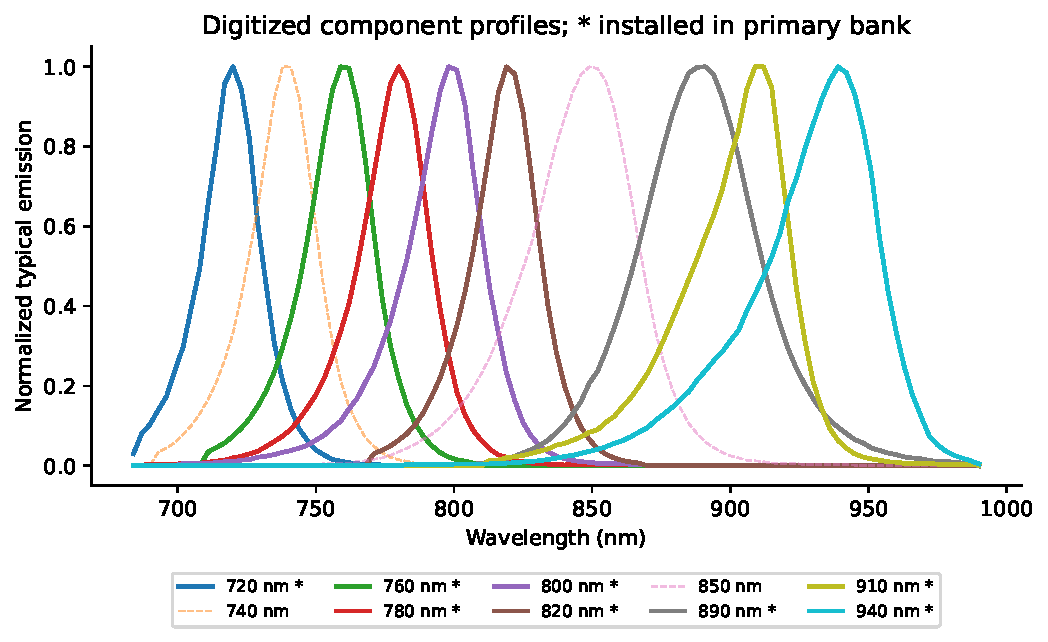
\includegraphics[width=0.92\linewidth]{figures/Figure_1.pdf}
\caption{Typical digitized response profiles used as fixed simulation assumptions. These define emulated finite-band inputs, rather than measured responses of a new scanner.}\label{fig:profiles}
\end{figure}

\subsection{Adaptive prediction and stopping comparison}
Let $f_S$, $f_B$ and $f_F$ denote predictions from the acquired subset, complete installed bank and rich spectrum. For assay $y$, write $e_U=|y-f_U|$. The proposed decomposition is
\begin{align}
g_{\mathrm{stop}}&=e_S-e_B, & g_{\mathrm{bank}}&=e_B-e_F, &
g_j&=e_S-e_{S\cup\{j\}}.
\end{align}
Negative values are retained. The bank-reference stopping target is $g_{\mathrm{stop}}>0.50$ pp; the matched rich-reference target is $e_S-e_F>0.50$ pp. The 0.50-pp material-correction threshold and 0.25/1.00-pp sensitivities are illustrative analysis settings, not agronomic requirements. Both references are fitted models. Consequently, $g_{\mathrm{bank}}$ mixes prediction-model differences with spectral differences and cannot be interpreted as irreducible optical loss.

The partial predictor is a masked 64/32-unit MLP. During fitting, each scan is paired with one uniformly sampled nonterminal mask per epoch; the full mask is never an MLP training target. Unread standardized inputs are set to zero independently of their actual value, with a separate availability bit distinguishing an observed zero. The complete bank uses autoscaled six-component PLS. The primary rich reference applies rowwise standard normal variate transformation, an 11-point second derivative with polynomial order two and 3-nm spacing, and autoscaled 12-component PLS. A compact CNN supplies a second reference, and an additional Walsh-architecture CNN is fitted under the present splits.\citep{walsh2024,walshthesis2024} Its preparation differs from the authors' concatenated spectral preparations; it is an adaptation, not an exact reproduction of a published score.

Three grouped inner folds generate out-of-fold predictions for the controller targets. All 64 masks containing the same initial pair are enumerated for target prediction; 63 nonterminal masks train the controller. Each scan receives equal total mask weight. The terminal partial prediction dispatches to the same fitted bank model, making $g_{\mathrm{stop}}=0$ at the endpoint. This hybrid endpoint is examined separately in the diagnostic study.

The two controllers have identical 64/32 architectures, initializations, training effort and signed action targets. Binary cross-entropy and standardized action-gain MSE have equal weight, with an auxiliary residual-error loss weighted by 0.25. Their binary stopping targets differ. Calibration uses reserved-population sequential paths. The policy continues when its calibrated gain probability exceeds a frozen threshold and chooses the highest-scored unread channel. Learned representations can still yield different action scores; the matched stopping-only comparison removes that coupling.

The benchmark scientific operating point is selected on development seasons to target four mean readings, with deterministic error and threshold tie-breaks. A separate engineering operating point applies the registered correction, bank-loss, error and budget constraints. If constraints fail, the registered fallback is labeled infeasible. Six bank proposals share the bounded search allowance. No threshold is adjusted using a later-season outcome.

Controls include residual-error stopping, a training-selected fixed order, random order, fixed lengths, and a two-step conditional-Gaussian look-ahead using only training-derived distributions for unread channels. The latter is a documented regression approximation, not an exact implementation of Valancius et al.\citep{valancius2024}. Static PLS, sparse-selection SVR and MLP controls use finite-band or ideal point-wavelength budgets. Seeds 7, 42 and 99 are retained for the specified stochastic contrasts; seed 42 is primary. Full comparisons, calibration, optical sensitivities and unsuccessful configurations appear in the supplement.

\subsection{Matched predictor and endpoint diagnosis}
The matched-predictor analysis fixes bank, acquired subset, order, core rows and evaluation rows. It compares the existing masked MLP with subset-specific autoscaled PLS, using $\min(6,|S|)$ components, and standardized ridge regression with $\alpha=10$. Hyperparameters are fixed. The two banks and all 64 reachable masks are retained. The common acquisition order starts with the endpoints and repeatedly selects the unread center farthest from acquired centers, with deterministic ties. This catalog-only order uses no assay information, but need not be predictively optimal.

At the seventh reading, the signed absolute-error change is decomposed per scan as
\begin{equation}
e_{\mathrm{MLP},7}-e_{\mathrm{PLS},8}
=\left(e_{\mathrm{MLP},7}-e_{\mathrm{PLS},7}\right)
+\left(e_{\mathrm{PLS},7}-e_{\mathrm{PLS},8}\right).
\end{equation}
The first term changes estimator at fixed readings; the second adds a reading within PLS. Neither term is forced positive. Separate logistic stopping models then compare the two binary targets using identical acquired-state features, consistent subset predictors and the fixed order. Each family uses its own complete-bank predictor for the bank-reference label, while the saved rich PLS reference remains common. They have no action head. Disjoint calibration groups fit isotonic mappings and select thresholds on the fixed grid $0,0.05,\ldots,1$; their tuning performance is not an evaluation result.

\subsection{Design-only subset and order selection}
The channel-design analysis reuses the same core, calibration and held-season predictions while reserving channel selection exclusively to the bank-design groups. For held seasons 1, 2 and 3, the design pools contain 9, 9 and 6 populations, comprising 998, 953 and 857 scans. Leave-one-design-population-out predictions score every reachable subset. All six bank/held-season designs are hash-locked before evaluating them on source prediction arrays.

For each bank and predictor family, the best subset at each depth 2--8 minimizes pooled scan MSE, with lexicographic ties. Independently, all 720 permutations of the six noninitial channels are evaluated. The selected nested order minimizes the sum of design MSE over depths 2--7, equally weighting depths. Independent fixed subsets need not be nested and are never represented as one adaptive path. PLS is primary; ridge and the uniform bank are sensitivities with their own selected designs.

The primary contrast is selected-order minus catalog-order RMSEP at exactly four readings. Separately selected fixed-four subsets are a secondary exact-budget contrast. Fixed-six is a prespecified sensitivity against the full eight-channel model, using an illustrative screen of no more than 0.25-pp RMSEP increase and at most six readings. This is a relative benchmark criterion, not a practical harvest-accuracy standard. The logistic stopping comparison is repeated on the selected nested orders with learner, objectives, calibration and threshold grid unchanged.

\subsection{Metrics, uncertainty and reproducibility}
For each evaluated season, RMSEP is $\sqrt{n^{-1}\sum_i(\hat y_i-y_i)^2}$. We also report MAE, signed prediction-minus-assay bias, reading count, early-stop coverage and the fraction of early stops with $g_{\mathrm{stop}}>0.50$ pp. Conditional rates retain their numerator and denominator; a zero denominator is undefined. Visited-state calibration is distinguished from final stopped-scan error.

The seasonal-benchmark primary estimand is RMSEP(bank-reference) minus RMSEP(rich-reference). A mean reading difference exceeding the registered 0.25-reading margin makes an unqualified equal-budget interpretation inappropriate. Frozen curves describe all planned thresholds without test-side optimization. In contrast, the fixed-four design comparison has exactly equal budgets by construction.

Paired 95\% percentile intervals use 1,000 resamples of complete harvest populations, with common resamples for both methods and seed 42. Season 5 has only two populations, so population-bootstrap intervals are suppressed. Intervals are conditional on the sampled populations, fitted models and selected designs; they do not describe future-season variation, unknown fruit identities or selection uncertainty. Multiple exploratory contrasts are reported without multiplicity-adjusted confirmatory claims. Design selection weights scans equally, so large populations have more influence; the held-season-1 design pool includes 958 of its 998 scans from season 3.

Saved partitions, fitted coefficients, frozen operating points and scored prediction tables support computational reproducibility. Tables and figures derive from these records, with numerical consistency checks against the retained predictions. Analysis code and supporting results are available through the Data availability statement.

\section{Results}
\subsection{Seasonal benchmark}
Table~\ref{tab:primary} reports both stopping objectives and strong local references. In season 4, the bank-reference and rich-reference controllers achieved RMSEP of 2.672 and 2.752 pp, using 3.096 and 2.365 mean readings. In season 5, their RMSEP was 1.997 and 2.171 pp, using 4.809 and 2.369 readings. The paired RMSEP differences were $-0.081$ and $-0.174$ pp, but the acquisition differences were $+0.731$ and $+2.441$ readings. Both exceed the 0.25-reading comparability margin. The season-4 RMSEP interval, $[-0.165,-0.014]$ pp, does not remove this budget difference; no season-5 population interval is reported.

\begin{table}[tbp]\centering\small
\caption{Seed-42 seasonal benchmark on seasons 4--5 from the same dataset. RMSEP is in dry-matter pp. ``Readings'' are simulated finite-band acquisitions; a rich-spectrum model uses 103 spectral variables, which are not equivalent physical LED pulses. Static four-channel models can use different subsets from a four-reading adaptive prefix.}\label{tab:primary}
% Generated from independently reconstructed frozen prediction exports.
\begin{tabular}{lrrrr}
\toprule
Method & S4 RMSEP & S4 readings & S5 RMSEP & S5 readings \\
\midrule
Two-reference, scientific & 2.672 & 3.096 & 1.997 & 4.809 \\
Single-reference, scientific & 2.752 & 2.365 & 2.171 & 2.369 \\
Two-reference, engineering & 1.261 & 7.942 & 1.244 & 8.000 \\
Complete-bank PLS & 1.232 & 8.000 & 1.244 & 8.000 \\
Full-spectrum PLS & 1.477 & -- & 2.229 & -- \\
Full-spectrum CNN & 1.503 & -- & 1.614 & -- \\
Uncertainty stopping & 2.364 & 4.908 & 1.657 & 7.028 \\
Random acquisition order & 2.662 & 3.171 & 1.828 & 5.100 \\
Two-step lookahead & 2.657 & 3.077 & 1.911 & 4.737 \\
Fixed four, masked MLP & 2.851 & 4.000 & 2.230 & 4.000 \\
Fixed four, PLS & 1.242 & 4.000 & 1.853 & 4.000 \\
Fixed four, sparse SVR & 2.361 & 4.000 & 1.530 & 4.000 \\
Adapted full-spectrum CNN & 1.276 & -- & 1.778 & -- \\
\bottomrule
\end{tabular}

\end{table}

The full-bank PLS errors were 1.232 and 1.244 pp. The rich PLS reference was less accurate in both later seasons, at 1.477 and 2.229 pp, showing why more spectral variables must not be equated with a better fitted predictor. The adapted Walsh-architecture CNN achieved 1.276 and 1.778 pp. Static four-channel PLS achieved 1.242 and 1.853 pp, while four-channel sparse SVR achieved 2.361 and 1.530 pp. Their different channel choices mean these comparisons alone cannot identify the cause of partial-prediction error.

Fixed ordering with stopping achieved 2.690 pp at 3.046 readings in season 4 and 2.013 pp at 4.641 readings in season 5. Two-step look-ahead achieved 2.657 pp at 3.077 readings and 1.911 pp at 4.7375 readings. These descriptive differences do not establish a consistent advantage for the proposed controller over simpler or alternative acquisition rules. Figure~\ref{fig:originalcurves} retains the complete frozen error--reading curves.

\begin{figure}[tbp]\centering
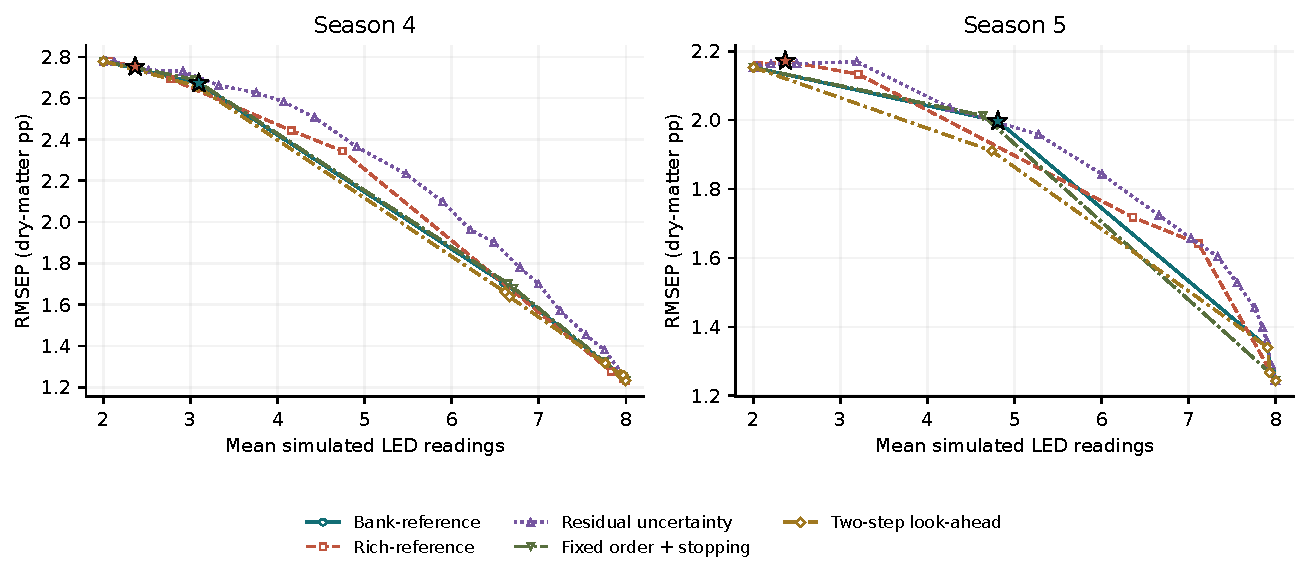
\includegraphics[width=\linewidth]{figures/Figure_2.pdf}
\caption{Frozen threshold curves by later season. Stars identify development-targeted scientific operating points. The curves expose achieved-budget differences; they are not retuned to select favorable test-set thresholds.}\label{fig:originalcurves}
\end{figure}

\subsection{Missed corrections and absolute prediction error}
At the scientific operating point, the bank-reference controller stopped early on 1,250 of 1,448 season-4 scans; 755 of those stops missed a material bank correction. In season 5 the corresponding counts were 199 of 320 and 106 of 199. Thus conditional missed-correction rates were 60.4\% and 53.3\%. For the rich-reference controller the rates were 819/1,384 (59.2\%) and 157/314 (50.0\%), with different early-stop coverage. Material bank losses occurred on 253/1,448 and 9/320 scans and were shared by policies using that bank.

No benchmark development candidate met the engineering constraints. The retained infeasible fallback acquired 7.942 and 8.000 mean readings, with RMSEP of 1.261 and 1.244 pp. It largely recovered full-bank accuracy by reading nearly the whole bank. The scientific point reduced readings but failed the illustrative relative-accuracy criterion in both seasons. Neither operating point demonstrated the intended combination of accuracy and acquisition savings across both seasons. State-level Brier scores, complete denominators, group errors, signed gains and agreement/error diagnostics are reported in the supplement; agreement between fitted references is not proof of low assay error.

\subsection{Predictor replacement did not explain the common-order gap}
At four identical primary-bank readings, masked-MLP RMSEP was 2.330, 1.740 and 2.457 pp for held development seasons 1--3. Subset PLS gave 2.372, 1.770 and 2.622 pp; ridge gave 2.372, 1.783 and 2.584 pp. Neither replacement improved these point estimates, and the corresponding paired intervals included zero. Equal-mask summaries over all four-channel subsets gave small, mixed changes. Consequently, the stronger static four-channel baseline in the seasonal benchmark cannot be attributed to predictor family alone.

The endpoint decomposition depended strongly on the bank and order (Table~\ref{tab:diagnostics}). In the primary bank, the final PLS measurement accounted for mean absolute-error reductions of 0.806, 0.291 and 0.906 pp, compared with estimator-switch components of 0.128, 0.086 and 0.101 pp. The final channel therefore retained substantial predictive value within the same estimator family. For the uniform bank, the measurement component was slightly negative in all three seasons, while estimator replacement accounted for the positive hybrid endpoint gain. These are fitted-pipeline effects, not universal statements about a seventh or eighth wavelength.

\begin{table}[tbp]\centering\small
\caption{Signed mean absolute-error reductions at the hybrid endpoint. Total equals estimator replacement at seven readings plus the final reading within PLS. Values and population intervals are in pp; negative components are retained.}\label{tab:diagnostics}
\resizebox{\linewidth}{!}{% Generated from independently reconstructed frozen prediction exports.
\begin{tabular}{llrrr}
\toprule
Bank & Season & Total & Estimator switch & Additional reading \\
\midrule
Primary & 1 & 0.934 [0.636, 1.269] & 0.128 [0.003, 0.239] & 0.806 [0.559, 1.055] \\
Primary & 2 & 0.377 [0.215, 0.569] & 0.086 [-0.004, 0.185] & 0.291 [0.154, 0.441] \\
Primary & 3 & 1.007 [0.715, 1.312] & 0.101 [-0.028, 0.228] & 0.906 [0.595, 1.197] \\
Uniform & 1 & 0.300 [0.070, 0.525] & 0.310 [0.076, 0.538] & -0.010 [-0.015, -0.005] \\
Uniform & 2 & 0.332 [0.193, 0.491] & 0.345 [0.209, 0.497] & -0.013 [-0.028, 0.004] \\
Uniform & 3 & 0.325 [0.003, 0.640] & 0.349 [0.029, 0.665] & -0.024 [-0.032, -0.016] \\
\bottomrule
\end{tabular}
}
\end{table}

\subsection{Channel design improved the exact-budget comparison}
Design-selected primary-bank PLS orders reduced four-reading RMSEP in every held development season (Table~\ref{tab:fixed}). The selected-minus-catalog differences were $-0.345$, $-0.600$ and $-0.586$ pp, with paired 95\% intervals $[-0.589,-0.118]$, $[-0.826,-0.382]$ and $[-0.800,-0.388]$. Both sides used exactly four readings with the same predictor family and fitting/evaluation rows. This controlled comparison identifies an avoidable channel-choice limitation in the earlier catalog order.

The independently selected fixed-four subset was 720, 890, 910 and 940 nm for each primary PLS design split. Its errors were 2.027, 1.171 and 2.036 pp. Despite the improvement over the catalog order, it met the illustrative full-bank-relative screen in only one of three seasons. Six separately selected channels achieved 1.215, 0.967 and 1.207 pp against full-bank values of 1.242, 1.293 and 1.207 pp, meeting that relative screen in all three seasons with exactly 25\% fewer simulated readings. The six-channel subsets differed between design splits; these results evaluate a selection procedure, not one universal device.

\begin{table}[tbp]\centering\small
\caption{Exploratory primary-bank PLS results. Four-reading contrasts use identical budgets. Six-channel subsets are selected separately using design populations; their scores are held-season results, not design minima. Errors and intervals are in pp.}\label{tab:fixed}
\resizebox{\linewidth}{!}{% Generated from independently reconstructed frozen prediction exports.
\begin{tabular}{lrrrrr}
\toprule
Season & Catalog 4 & Designed 4 & Selected 6 & Full 8 & Designed 4 minus catalog 4 \\
\midrule
1 & 2.372 & 2.027 & 1.215 & 1.242 & -0.345 [-0.589, -0.118] \\
2 & 1.770 & 1.171 & 0.967 & 1.293 & -0.600 [-0.826, -0.382] \\
3 & 2.622 & 2.036 & 1.207 & 1.207 & -0.586 [-0.800, -0.388] \\
\bottomrule
\end{tabular}
}
\end{table}

\begin{figure}[tbp]\centering
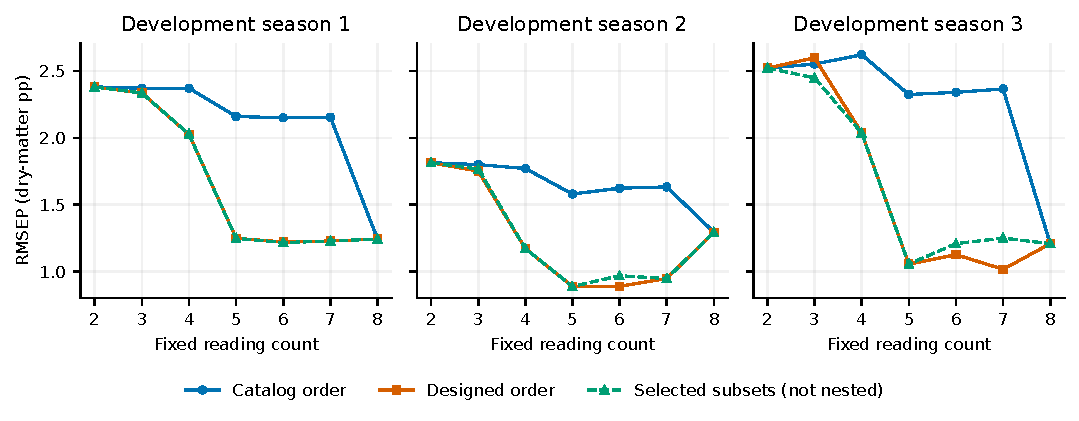
\includegraphics[width=\linewidth]{figures/Figure_3.pdf}
\caption{Fixed-budget results in the three held development seasons. The study evaluates design selection and acquisition effort without selecting a favorable held-season threshold. All displayed data remain exploratory because the development seasons had been examined in earlier stages.}\label{fig:fixed}
\end{figure}

The uniform-bank and ridge sensitivities did not consistently reproduce the primary-bank PLS improvement. For example, designed four-reading PLS on the uniform bank had RMSEP 2.343, 1.712 and 2.505 pp, compared with catalog-order values 2.286, 1.732 and 2.356 pp. Thus a favorable result on one bank/predictor combination is not a general guarantee of order optimization. Complete family/bank results and selection stability are provided in the supplement.

\subsection{The improved order did not rescue the stopping objective}
With the design-selected order and subset PLS held fixed, the bank-reference stopping objective had higher RMSEP than the rich-reference objective in all three development seasons (Table~\ref{tab:stopping}). The differences were $+0.039$, $+0.046$ and $+0.399$ pp. Their intervals were $[-0.027,0.138]$, $[0.007,0.091]$ and $[0.079,0.777]$ pp. Achieved mean-reading differences were within the registered 0.25-reading margin in all three cases, although not exactly zero. This provides no evidence for the proposed objective's advantage under the controlled learner and order.

\begin{table}[tbp]\centering\small
\caption{Exploratory stopping-only comparison on the designed primary-bank PLS order. Differences are bank-reference minus rich-reference; positive RMSEP differences favor the latter. Budgets meet the registered comparability margin but are not exactly equal.}\label{tab:stopping}
\begin{tabular}{lrrrrl}
\toprule
& \multicolumn{2}{c}{Bank-reference} & \multicolumn{2}{c}{Rich-reference} & Paired RMSEP difference \\
Season & RMSEP & Readings & RMSEP & Readings & Estimate [95\% CI] \\
\midrule
1 & 2.002 & 4.020 & 1.963 & 4.115 & 0.039 [-0.027, 0.138] \\
2 & 1.215 & 3.839 & 1.169 & 4.004 & 0.046 [0.007, 0.091] \\
3 & 2.241 & 3.747 & 1.842 & 3.821 & 0.399 [0.079, 0.777] \\
\bottomrule
\end{tabular}

\end{table}

Adaptive engineering points used fewer readings than fixed-six but had higher RMSEP. That is an observed accuracy--effort trade-off, not adaptive superiority at equal cost. Frozen threshold curves and every prespecified fixed depth are retained. We do not choose a new operating threshold after inspecting the held-season outcomes.

\begin{figure}[tbp]\centering
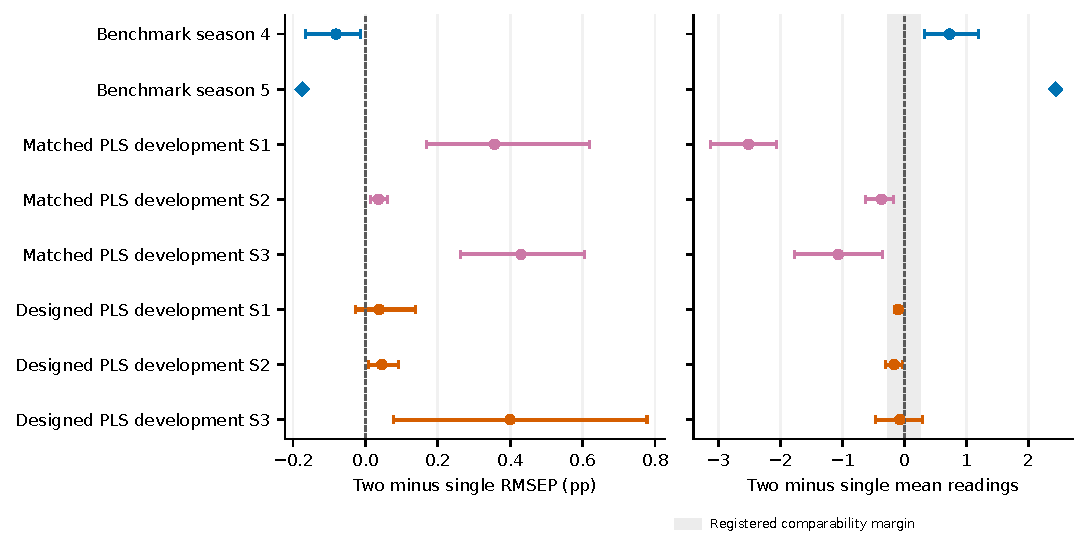
\includegraphics[width=\linewidth]{figures/Figure_4.pdf}
\caption{Paired contrasts for the seasonal benchmark, matched-predictor diagnosis and designed-order comparison. These comparisons are shown separately and are not pooled as independent repetitions. Signs and achieved reading differences accompany RMSEP effects; season 5 has no population interval.}\label{fig:contrasts}
\end{figure}

\section{Discussion}
\subsection{What the dataset establishes}
The analysis separates three claims that could otherwise be conflated. First, the bank-reference controller's lower errors came with substantially higher acquisition budgets than its matched objective comparator. Second, controlling the predictor at identical subsets did not show that the masked MLP alone caused the weak partial-scan performance. Third, choosing better channels improved four-reading prediction on the primary bank, while the proposed stopping objective still did not improve the controlled comparison. Taken together, the evidence favors careful fixed design over additional controller complexity for the tested setting.

The favorable fixed-six result is useful but narrow. It is a relative comparison against an eight-channel fitted reference, with 25\% fewer simulated readings. It does not establish that six is globally optimal, that the six wavelengths should be identical across seasons, or that the absolute errors satisfy a harvest requirement. Its selection is confined to the existing eight-channel banks and initial pair, and its results are conditional on the chosen PLS family and design populations. The uniform-bank and ridge sensitivities show why those qualifications matter.

The loss-gap decomposition remains a useful diagnostic description even when it does not yield a better policy. It exposes missed opportunities to use the installed bank and disagreements between fitted references. It should not be relabeled as a new general early-exit principle, nor treated as a measurement of irreducible information loss. The full-bank model outperforming rich PLS in later seasons is direct evidence that reference quality and fitting choices affect its interpretation.

\subsection{Limitations}
The later-season benchmark is reused, and the development seasons were examined repeatedly. The predictor and channel-design analyses therefore supply explanatory, exploratory evidence rather than independent confirmation. Group separation prevents direct population overlap within the registered fits, but cannot erase researcher exposure to previous results. Bootstrap intervals condition on fitted choices and sampled populations; they do not quantify that development history.

Unknown fruit identities prevent fruit-level counts and averaging of known repeat scans. Population grouping is a conservative documented substitute, not proof that every possible dependence is captured. The small and uneven design pools also limit selection stability; in one fold almost all design scans come from one source season. Season 5's two populations provide descriptive evidence without a population-level interval. A bounded catalog and model search cannot establish the best possible sensor or regressor.

All sparse channels are emulated from full spectra using fixed typical response curves. The conventional log-base interpretation, flat detector/reference response and truncated spectral support are explicit assumptions. The present study establishes numerical behavior under those assumptions. It does not measure physical scanner performance. The conclusions apply to the observed dataset under the specified simulation assumptions.

For the same reason, a dry-matter prediction is not itself a validated instruction to pick a mango. Harvest timing remains a motivation, while the manuscript's demonstrated endpoints are prediction error, acquired-channel count and stopping behavior. No maturity cutoff, field outcome or economic benefit is inferred from labels that the dataset does not contain.

\subsection{Final six-channel model and reproducibility}
For reproducible sparse inference, a final six-channel research candidate was selected using all 10,243 development scans and 94 leave-population-out folds over the 15 allowed six-channel subsets containing the fixed endpoints. The selected nominal centers are 720, 760, 820, 890, 910 and 940 nm. A six-component PLS model, an eight-channel PLS comparator and a rich-spectrum PLS comparator were fitted and frozen with portable coefficients, response weights and exact feature schemas. Using as many PLS components as input channels imposes no component-count reduction and is not evidence of a new dimension-reduction method.

The final model's selection minimum is tuning evidence; it is not assigned the accuracy of the fold-specific fixed-six models in Table~\ref{tab:fixed}. The public software provides sequential-acquisition replay and a six-input prediction interface, neither of which consumes hidden full-spectrum information at sparse inference. The final six-channel model has no separate accuracy evaluation on seasons 4--5.

\section{Conclusion}
On this public mango dataset, the proposed bank-reference stopping objective did not demonstrate an advantage over a credible rich-reference alternative. The seasonal benchmark comparison was confounded by unequal achieved reading budgets, and controlled follow-ups did not support the objective after predictor and order effects were separated. Design-only fixed-channel selection substantially improved the exact four-reading comparison on the primary PLS bank, and separately selected six-channel subsets retained full-bank-relative accuracy in the three exploratory seasonal folds. These findings support a fixed-acquisition research baseline and clarify where adaptive complexity failed to add value. They establish a completed dataset-based empirical result, with no claim of validated harvest decisions or measured hardware savings.

\section*{Acknowledgements}
OpenAI Codex was used for research-code implementation and debugging, execution and reporting assistance, literature-source checking, manuscript drafting and revision, and preparation of the LaTeX submission files. The empirical measurements originate from the cited public mango dataset. Spectral-response emulation is described in the methods; numerical figures are generated from recorded analysis outputs. Generative AI was not used to fabricate mango observations or to create images presented as measured scientific evidence. \HumanReviewStatement

\AdditionalAcknowledgements

\section*{Author Contributions}
\AuthorContributions

\section*{Statements and Declarations}
\subsection*{Ethical considerations}
Not applicable. This computational reanalysis uses an openly released mango spectral dataset and involves no human participants, personal data or animal experiments. No new fruit collection or field intervention was conducted for this study.

\subsection*{Consent to participate}
Not applicable.

\subsection*{Consent for publication}
Not applicable.

\subsection*{Declaration of conflicting interest}
\ConflictStatement

\subsection*{Funding statement}
\FundingStatement

\subsection*{Data availability}
The source dataset, \emph{Mango DMC and spectra Anderson et al.\ 2020}, version 3, is available under CC BY 4.0 at \url{https://doi.org/10.17632/46htwnp833.3}. The supplementary document reports complete operating-point results and detailed methods. The manuscript-source package contains LaTeX sources, figures, supporting result tables and a build script. Model-training code, frozen model checkpoints, the replay application and the candidate command-line interface remain in the preserved research workspace; they are not bundled into the manuscript-source archive. \SoftwareAccessStatement

\section*{Supplemental material}
Supplemental material for this article comprises the supplementary methods and complete operating-point results, including the full comparison tables, unsuccessful analyses and data/code availability. A separate description file identifies the supplied supplemental item.


\bibliographystyle{jnirs_sagev}
\bibliography{references}
\end{document}
